\clearpage
% Introduction.tex
\chapter{Literature Review}
\label{chap:introduction}

\section{ Assistive Robotics in Healthcare}
\label{sec: Assistive Robotics in Healthcare}

Medication adherence is to be one of the most significant  challenges in modern healthcare systems, especially among elderly populations, patients with chronic diseases or cognitive issues, and those who require long-term therapeutic regimens. Non-adherence to  medications has been associated with increased rates of hospitalization, avoidable complications, reduced quality of life, and a substantial rise in healthcare costs. According to the World Health Organization (WHO), approximately 50\% of patients in developed countries do not take their medications as prescribed~[1]. In developing countries, the situation is even more critical due to issues such as lack of education, poor access to healthcare, and limited infrastructure.

Medication non-adherence can arise from many reasons, i.e. errors of omission (forgetfulness), cognitive deficits, complexity of medication regimens, adverse drug reactions, low literacy or health literacy, and lack of incentives. Sociocultural elements can also drive drug non-adherence, such as stigma, belief in traditional remedies, and lack of trust in pharmaceuticals~[2].

Smart medication dispensers are a viable solution to address many of these barriers. Smart medication dispensers automate the dispensing process and reduce memory dependency, through the use of IoT, artificial intelligence (AI), biometric security, and real-time monitoring. Smart medication dispensers have gone beyond single functionality (simple pillboxes) to intelligent and IoT-enabled systems that can connect and communicate with patients and caregivers~[2].

\begin{figure}[h!]
    \centering
    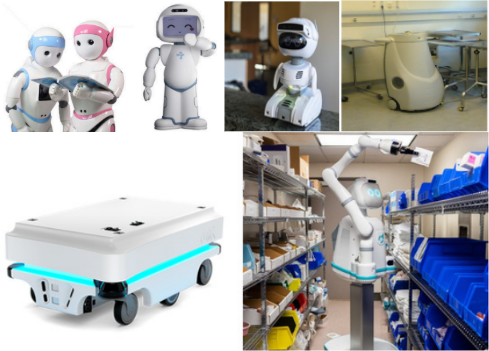
\includegraphics[width=0.8\textwidth]{Medora_thesis (1)/pics/thesis/Servicerobot.png}
    \caption{Service robots in Healthcare Sector~[2]}
    \label{fig:healthcarerobots}
\end{figure}

Some advanced implementations have incorporated robotic systems with temperature sensors, voice interact modules, and audiovisual communication for limited human contact and remote care, especially during a pandemic. Yet, there are still challenges in calibration, navigation, and speech recognition in rapidly changing care settings~[3].

For technology to have general application, it must utilize human-centered design. Research has shown that modern dispensers also need to be intuitive and designed for wide accessibility, especially for older adults or individuals with cognitive limitations~[4]. MediBot-designed robots provide more than old pill dispensers; they offer health monitoring (in and out), medication reminders, encourage emotions and support independent living. Acceptance of the robots depends on their perceived usefulness, perceived ease of use, user experience, and appearance~[5].

This research supports the democratization of assistive technology by developing a low-cost, open-source software and hardware system utilizing computing technology, such as Raspberry Pi, OpenCV, and TensorFlow. The resulting system will be low-cost, configurable to individual users, and flexible for a variety of care settings~[6].

In summary, this chapter identifies the technological development, benefits, limitations, and designer priorities for smart medication dispensers and has laid the groundwork to integrate a validated technology to create a functional and inclusive system~[7].



\section{Historical Background and Evolution
}
\label{sec:Historical Background and Evolution
}

Historically, drug control has relied on manual systems such as pillboxes, paper-based medication calendars, and visual checking by caregivers or clinicians . These manual devices, although functional to some degree, were neither accurate nor reliable. Moreover, they did not possess any kind of real-time monitoring or alerting mechanism, thus unable to send reminders or alert users or caregivers in the event of a missed dose.
At the end of the 20th century, there were simple electronic assistive devices. These were programmable watches, alarms, and digital reminders. Although revolutionary for the time, these devices required a great deal of user input and offered very little customization and feedback.
Semi-automatic dispensing drug machines initially came to the scene in the early 2000s. They were made up of rotating pill trays, sound alert, and programmable digital countdown timers. Electronic models such as the Weekly Electronic Pill Dispenser and the Pill-Mate Medicine Reminder were easy to operate and reminded users of their dosage regimen[8] . However, they did not have usable confirmation or caregiver alerts for missed doses. As microcomputing, electronics, and telecommunications evolved, scientists and engineers started adding sensors, controllers, and wireless communication to medication dispensers. In the 2010s, smart technology and healthcare began to intersect, leading to a new generation of connected dispensers. Devices like MedMinder, TabSafe, and Philips Medication Dispenser introduced secure lock compartments, cellular connectivity, and remote monitoring features. 

The latest generation of smart dispensers, such as PillGood, RxPense, and internet-of-things-based pill managers, now includes facial recognition, cellular connectivity, cloud storage for information, and interactive feedback. Besides dispensing medication, they collect data, track usage patterns, and intervene if issues arise. Their development highlights how health technology contributes to viewing medication adherence as both a personal and systemic challenge.


\section{ Key Technologies in Smart Healthcare}

\subsection{ Microcontrollers and Hardware}
Almost all of the medical assistive devices made today consist of a microcontroller as the main hardware component (e.g. Arduino, Raspberry Pi, BeagleBone, etc.). As they are low-cost and programmable, these platforms can perform essential functionality, such as tracking time of day, controlling motor activity, executing user interface tasks, integrating a range of sensors, communicating with other peripheral hardware in real-time, and a host of other capabilities.  The modular and flexible designs allow for custom designs that easily scale to the needs of many healthcare settings.

Typically, mechanical tasks (e.g. dispensing medication or performing other types of movements such as rotating camera modules, sound alerts, etc.) are handled by servo motors, which operate based upon electrical programming to achieve hardware movement and/or shifting. Real-Time Clock (RTC) modules allow precise scheduling in consideration for those who may rely upon our devices for medication reminders and time-dependent healthcare monitoring tasks [11]. Sensors such as IR and ultrasonic modules can assist with detecting a user being present, estimating distance, and verifying medications being picked up/touched.

For the devices to engage a user, displays (e.g. OLED/LCD), capacitive touchscreens, buttons, LED, and audio sounders can be used to confirm interaction [12]. More sophisticated devices may incorporate advanced technologies such as voice synthesis for spoken alerts, haptics from vibration motors, and facial recognition for customizing interactions and access.
Also, many systems include battery management systems (BMS) and uninterruptible power supply (UPS) modules to help provide important reliability to confirm services are not disrupted, especially when deployed in rural communities or environments with limited resources. Both BMS and UPS systems provide redundancy and decrease reliance on continuous supply of electricity making the assistive robot more amenable to real-life broader deployment contexts.

\subsection{ Connectivity and Notification}
To enable real-time monitoring of compliance, dispensers are often equipped with GSM, Wi-Fi, or Bluetooth communications modules. GSM modules send SMS alerts to caregivers or family members when medication has not been taken or taken improperly [13]. Wi-Fi modules allow remote updating of the dosage schedule as well as monitoring of usage over time through cloud-based dashboards [14].
Bluetooth Low Energy (BLE) connectivity is becoming increasingly popular due to its low power consumption and mobility app integration. Dispensers can be synchronized with smartphones and wearable health devices to offer an improved integrated health management experience.
NFC (Near Field Communication)[15] is utilized in some systems for quick user authentication or caregiver sign-in, especially in multi-occupancy settings.Additionally, MQTT (Message Queuing Telemetry Transport) protocols are widely used in IoT-integrated dispensers to allow lightweight, secure, and real-time connectivity to cloud servers.


\subsection{ Biometric and Smart Authentication}
Safety of the patient is paramount when giving out medication. To ensure that drugs reach only authorized people, modern systems implement biometric verification such as fingerprint scanners, RFID tags, and facial recognition[16]. As an example, Haar Cascade face detection along with user enrollment and user profile management is employed by PillGood dispenser. Similarly, RFID-based systems allow pre-approved individuals to use only pre-approved medication to which they are assigned.
In more sophisticated systems, facial analysis is being explored for detecting emotions to quantify patient mood and identify warning signs such as depression or confusion[9],[17]  symptoms commonly found with non-compliance with medication.
Voice recognition is even being explored as a security function[18]. Multi-modal function is being used in some prototypes for high applications such as hospitals or psychiatry clinics.


\section{ AI and IoT Integration}
The collaboration of Artificial Intelligence (AI) and Internet of Things (IoT) in medical dispensers has changed the way medicines are administered and managed, especially for elderly and chronic patients. Together, AI and IoT technologies facilitate the smart dispenser functions, adding automation, real time monitoring, and remote management for medication regimens [19]. IoT devices with Wi-Fi and GSM [20] modules permit these dispensers to be connected to the internet and communicate significant information to healthcare providers or caregivers. Patient compliance may be monitored remotely, and reminders or alerts can be activated when doses are missed [20].

AI is at the forefront by checking on patient behaviors and patterns in their consumptions of medications to make data driven decisions of the timing of doses and compliance [21]. Some systems actually utilize advanced AI capabilities like voice command detection, and face recognition to ensure the identity of a user, such that medications are distributed safely and zero waste to a correct individual. 
In addition to its dispensing function, AI-based systems will probably use mobile apps or LCD screens to provide real-time feedback, instructions, and alerts[22]. Alerts might be conveyed to patients via SMS, buzzers, or application alerts, thereby minimizing the possibility of human error and increasing medication adherence[23]. Moreover, AI algorithms analyze information from IoT sensors to build context regarding patient behavior and the effectiveness of prescribed drugs which can be either communicated back to the medical staff to enhance clinical decisions.
\begin{table}[htbp]
\centering
\caption{Comparison of Two Medical Assistance Robot Systems}
\label{tab:robot_comparison}
\begin{tabular}{|p{1.5cm}|p{3cm}|p{5cm}|p{5cm}|}
\hline
\textbf{Citation} & \textbf{ Algorithm} & \textbf{Working Process (Figure)} & \textbf{Picture} \\
\hline

\cite{24} &

- Machine Learning (Face Recognition) using OpenCV \newline
- Image Processing \newline
- Raspberry Pi for control \newline
- IoT-based remote monitoring 
& 
- Raspberry Pi captures patient’s face via camera \newline
- OpenCV matches the face with stored database \newline
- If authenticated, servo motor dispenses medicine \newline
- Buzzer confirms operation \newline
- IoT sends adherence data to caregivers \newline

& 
\raisebox{-1\height}{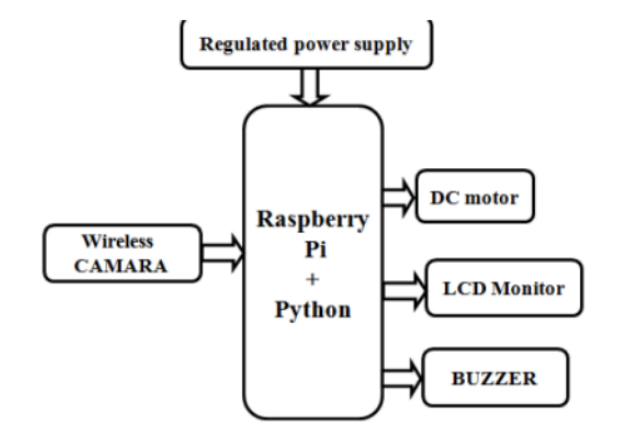
\includegraphics[width=5cm]{Medora_thesis (1)/pics/thesis/t2.png}} \\
\hline

\cite{25} &

- Autonomous Navigation (Line following) \newline
- IoT \& GSM Communication \newline
- AI-driven Object Detection \newline
- Medical Sensors for Monitoring \newline
- Disinfection Systems 
& 
- Robot follows predefined path to deliver medicine/food \newline
- Live monitoring through Wi-Fi camera \newline
- Communication via GSM for alerts \newline
- Health data from sensors sent to cloud \newline
- Sanitizer dispenser and waste collection unit maintain hygiene \newline

& 
\raisebox{-1.5\height}{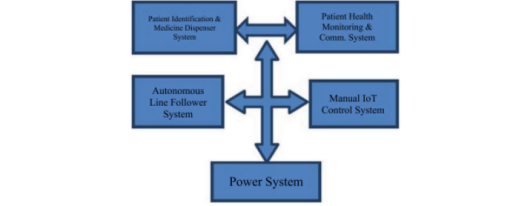
\includegraphics[width=5.7cm,height=3cm]{pics/thesis/t1.png}} \\
\hline

\end{tabular}
\end{table}

The integration also facilitates cloud storage of information, allowing easy access to drug history and distant consultations. Real-world use cases of such a system include AI-enabled dispensers like Arduino [25]or Raspberry Pi being controlled by a microcontroller that is coupled with AI for detecting medicine dispensing time and real-time user interaction. Not just the dispensing becomes automated when AI and IoT are integrated within medicine dispensers, but health delivery becomes wiser, more secure, and efficient.


\section{Human-Centered Design Consideration}

Human-centered design (HCD) is crucial in creating automated medication dispensers, especially for elderly or physically impaired users. It is important to design for usability, accessibility, and flexibility to meet varying user needs and cognitive skills.

As we discussed, a strong aspect of an HCD approach (Human Centered Design) is employing users as active participants throughout the design and development process. Specifically, when we carry out our initial research on the user, we are determining their context, the issues with adhering to prescribed medications, and their physical limitations, including those that impact blind people or those with dexterity issues. The findings from the user-based research stage will give form to the design, which will contain mostly key elements such as the point-and-click interface, visual and auditory cues, and simple mechanical motions.

Ergonomic principles that are properly employed (i.e. appropriately sized buttons, high contrast contrast display, easy to read fonts and voice prompts) can encompass often overlooked ways of engaging users with limited technology skills. We have also learned the importance of culturally sensitive approaches to the introduction of new technologies, which can vary based on geographic area, rural vs urban areas, or socioeconomic status.



Key design principles for smart medication dispensers include:

\begin{itemize}
    \item \textbf{Large buttons and screens} to accommodate users with low vision.
    \item \textbf{Voice-guided interfaces} for individuals with cognitive or visual impairments.
    \item \textbf{Minimal setup complexity}, ensuring plug-and-play operation for ease of use.
    \item \textbf{Tactile and audible feedback} to confirm successful interactions.
    \item \textbf{Multilingual support and culturally aware design} for broader global accessibility.
    \item \textbf{Fail-safe mechanisms} that prevent medication from being dispensed at incorrect times.
\end{itemize}


Alongside those principles, privacy and autonomy are also cornerstones in human-centered design. The system should give users agency over medication management and provide autonomy while alerting caregivers when there is non-adherence; at the same time, it is vital that any disclosures regarding health-related data meets ethical and legal guidelines, i.e., informed consent and robust data protection.

In conclusion, the effectiveness of smart medication dispensers is also dependent on a caring user-centered design that assists by being a user-centered solution that addresses actual needs in use and a real-world context.
\section{ Real-World Application}

\subsection{Home-Based Smart Pill Dispensing Technologies}
Smart medicine dispensers are essential in home care settings. They help older adults and people with chronic conditions live independently. These devices are small, affordable, and easy to use. They allow users to manage their medication schedules with assistance from caregivers. Some prescriptions come with adjustable schedules and pre-set alarms. However, some models require users to handle their medication timing with little help from home care providers.

Smart dispensers use GSM or Wi-Fi, although not all do, to send real-time notifications to a caregiver or family member about missed doses or low medication supplies. The ability to notify users of missed medications allows for timely support, which improves patient adherence and care. This, in turn, can reduce complications linked to medication management.

Additionally, smart dispensers offer features like audible reminders, locked compartments to lower the risk of overdose, and the ability to sync with an app or cloud dashboard. They often automate data collection and integrate with medical analytics. They can also alert multiple contacts, including emergency responders, after a set number of missed doses. These capabilities enhance patient safety and lighten the load for caregivers while empowering users to take charge of their health care needs.

\begin{table}[h!]
\centering
\renewcommand{\arraystretch}{1.5}
\begin{tabular}{|>{\raggedright\arraybackslash}m{3.5cm}|>{\raggedright\arraybackslash}m{4.5cm}|>{\raggedright\arraybackslash}m{5cm}|>{\centering\arraybackslash}m{3cm}|}
\hline
\textbf{Citation} & \textbf{Algorithm / Application} & \textbf{Actions / Functions} & \textbf{Robot Image} \\
\hline
\textbf{[26]} 
& 
- Real-Time Monitoring \newline - Activate Pill Dispensing \newline - GSM Module 
& 
- Scheduled Medication Dispensing \newline - Missed Dose Notification \newline - Medication Adherence Log 
& 
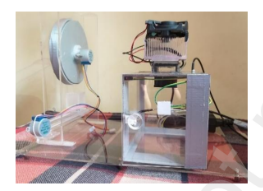
\includegraphics[width=2.5cm]{Medora_thesis (1)/pics/thesis/dt2.png} \\
\hline

\textbf{[27]} & 
- Real-Time Monitoring \newline - Scheduling \& Cloud Sync 
& 
- System Initialization \newline - Scheduled Dispense \newline - Notification and Escalation 
& 
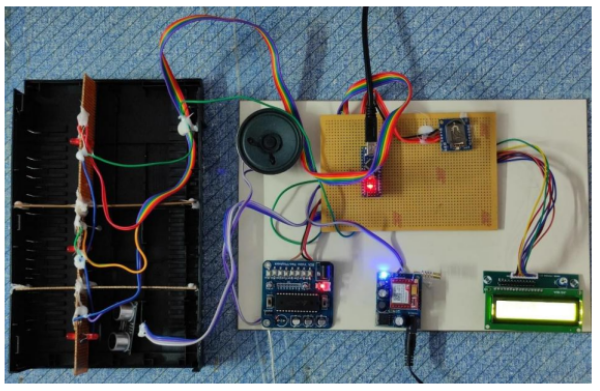
\includegraphics[width=2.5cm]{Medora_thesis (1)/pics/thesis/table2.png} \\
\hline
\end{tabular}
\caption{Comparative Analysis of Smart Medication Dispensers}
\end{table}




\subsection{ Elderly and Institutional Care}

In elderly care homes and long-term care facilities, addressing social isolation, medication management, and emotional well-being are important challenges. To address these limitations, various robotic systems have been employed. One form of long-term care robot that has emerged is the telepresence robot. Telepresence robots will help maintain social engagement and remote monitors for health conditions. The telepresence robot allows elderly individuals to communicate with their caregivers, family members, or physicians through video links. This reduces cognitive decline associated with loneliness, and provides health consultations without the need to physically be there. Hear during the pandemic, the telepresence robot was helpful at avoiding exposure while assuring the continuity of care and emotional connection [28].

Another noteworthy example is \textit{Paro}, a robotic baby seal designed for therapeutic interaction. Paro has tactile sensors, microphones, and artificial intelligence that allow it to respond to touch, light, sound, and temperature. It mimics the behaviors of a live animal, such as blinking, making soft sounds, and nuzzling. This provides comfort and companionship to elderly users. Studies have shown that interacting with Paro can reduce stress, agitation, and feelings of loneliness in older adults, particularly those with dementia [29]. Unlike standard social robots, Paro is used specifically for animal-assisted therapy in settings where live pets are impractical or not allowed. These systems not only help with practical functions but also create emotional presence, which is very important and often overlooked in older adult care. By using features like live feedback, empathetic responses, and therapeutic engagement, robots like telepresence robots and Paro promote better mental health, regulate mood, and enhance quality of life in older adult residents [30].

\begin{figure}[h]
    \centering
    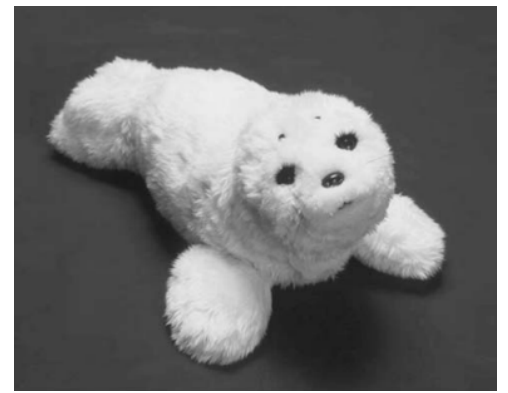
\includegraphics[width=0.5\textwidth]{Medora_thesis (1)/pics/thesis/Paro.png} % Replace with your actual image filename
    \caption{Therapeutic robot Paro used in dementia care [31]}
    \label{fig:paro}
\end{figure}

At the same time, newer emotion awareness technologies like facial expression detection, vocal tone recognition, and biometric surveillance are being used to create more personalized music-based interventions for people with dementia. By identifying a person's emotional state, such as agitation, sadness, or calmness, the system can play specific songs that help with relaxation, improving mood, or enhancing cognitive function by triggering sound playlists [32]. Research shows that emotion-aware music therapy improves mood and reduces anxiety. It also helps with memory recall and interaction with others in people with dementia, creating a user-focused and non-drug approach.

Our proposed robot builds on these insights by combining health monitoring and emotional awareness. Although it does not yet provide the therapeutic features of Paro or the high-quality video communication of telepresence robots, it includes facial recognition, emotion detection, temperature sensing, voice interaction, and medication reminders. This creates a single platform for everyday support in both home and institutional settings [33].
\subsection{ Pharmacies and Clinics}

In hospitals and pharmacies, medication dispensing systems have transitioned from bulk distribution methods to an emphasis on accuracy, safety and integration into the broader healthcare workflow. New advancements in robotic dispensers, including automated oral unit dose distribution systems, intravenous (IV) medication robots have demonstrated meaningful advancements in reducing dispensing errors, maintaining sterility, and improving pharmacy workflow. Robotic systems that utilized barcode verification of medications, along with AI tracking features, decreased medication errors, and increased dispense times, allowing the pharmacist to spend more time providing clinical care and counseling patients. Though systems are automated, human verification remains critical in managing mechanical challenges and ensuring systems are faultless. 
In addition, robotic dispensers can be integrated with hospital information systems and in-house prescription databases. Integrating robotic dispensers strengthens medication management with more transparent reporting and control of inventory. Intelligent intravenous dispensing robots mitigate contamination risk and improve dosing accuracy within sterile environments which improves patient safety under critical care situations. However, obstacles like technological failures, maintenance, training personnel still impede widespread adoption.
Automated dispensing machines (ADMs) are present in more hospital pharmacies around the world with the aim of reducing human error, increasing capacity for storage, and optimizing staff time. Although ADMs reduce dispensing errors significantly, especially when not selecting drug content, there is potential for errors in labeling as well. The impact on time for processing prescriptions has been variable. While automation has improved retrieval time for items, bottlenecks remain in labeling and dispensing due to manual checks. ADMs are typically associated with an increase in medication storage and utilization of space. While pharmacy staff may see it as a reliable option that adds to positive job satisfaction, staff perceptions of reliability and job satisfaction vary [37]. 
Limited comparative studies across different ADM systems highlight systemic benefits and a lack of understanding difference between benefits of current system or previous system [37].
Pharmacy staff appear to have a positive perception of robotic dispensing systems particularly with respect to job security and renewed focus on clinical service. However, pharmacy staff have observable dissatisfaction with management decisions and the process of inclusion with medication processing changes that should emphasize improve communication and partnership during integration. Very clear communication and training for all staff members ensures that information is shared.


In addition to hospital pharmacies, humanoid robots and automated dispensing technologies are also being evaluated for use in community pharmacies and in industrial pharmacies. Lessons learned from the hospitality sector— in which humanoid robots have productive interaction with customers—provide models of enhanced patient engagement, patient questions about medications, and dispensing efficiencies within pharmacy contexts. These robots and automated dispensing systems, which use artificial intelligence and machine-enabled learning, offer the potential to relieve human workloads, reduce errors, enhance inventory management capabilities, and decrease liability associated with encountering counterfeit and commonly misbranded drugs. Nonetheless, considerations regarding initial investment—both ethically and with respect to obtaining government approval— must be addressed to establish safe and effective applications [38].
Examples of operational improvements when robotic dispensing machines (like ROWA systems) are implemented in community pharmacy show improvements in terms of cost per transaction, personnel cost reductions, and capacity to improve over-the-counter and pharmacy sales when pharmacists are freed up to provide patient consultation. Even though implementations have incurred high initial costs, many pharmacies have reported realizing stabilizing or even reduced costs within one year of implementing robotic dispensing technologies, to which operational costs associated with personnel and inventory management are continuously modified and optimized [39].
In home health care services, automated dose dispensing (ADD) robots are already associated with improved medication adherence and ease of use, but mixed opinions exist among health care professionals about interacting with patients and the initial need for ADD robots [40]. Additionally, implementing electronic prescribing and robotic dispensing for hospitals has improved efficiencies of staff, redirected staff resources, produced considerable cost savings, and removed dispensing errors. These outcomes underscore the importance of integrated technology structures in pharmacy practice [40]. 
Robotic systems and AI technology for medication management are also being developed to directly interface with patients. Health care robots that share information with medication entry analysis software (e.g., RoboGen) work to independently record automatic prescription entry, reminders, and patient monitoring; this is appropriate, particularly for elderly or chronically ill patients. This family trees leverages computer vision and machine learning methods (e.g., CNN and YOLO) for recognizing medications and performing each task that supports pharmaceutical logistics and decreases errors [41].In the meantime, robotic pharmacies, and AI-enabled inventory systems are employed for precise medication management, packaging, and adherence tasks [42]. Similar to this, medical dispensing systems using IoT will automate patient's medication schedules and send reminders, dispense water and remotely monitor patients for adherence while reducing burdens on caregivers [43]. 
In summary, pharmacies and clinics are increasingly implementing intelligent robotic dispensing systems that improve safety and operational efficiencies. These systems will blend AI-enabled patient monitoring, IoT sanitization, and robotics allowing for a paradigm shift in personalized care, infection control and clinical outcomes.
\begin{table}[htbp]
\centering
\caption{Smart medical bot Implementations in Healthcare and Pharmacy Settings}
\label{tab:library_interaction}
\begin{tabular}{|p{1.5cm}|p{7cm}|p{3cm}|p{3cm}|}
\hline
\textbf{Citation} & \textbf{Application} & \textbf{System} & \textbf{Structure} \\ 
\hline

\cite{44 ,45} & 
An autonomous robotic system designed for elderly care that dispenses medication based on scheduled routines. It ensures timely delivery, navigates through home environments, and enhances medication adherence with real-time alerts and safe mobility. & 
Infrared tracking, obstacle avoidance, schedule management & 
\multicolumn{1}{|c|}{\raisebox{-1\height}{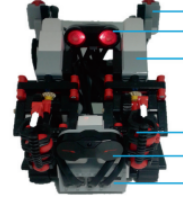
\includegraphics[width=3cm]{pics/thesis/TB1.png}}} \\
\hline

\cite{46} & 
A robotic system for hospital pharmacies that automates drug storage, retrieval, and dispensing to improve accuracy, inventory control, and operational efficiency. &
Prescription verification, barcode scanning, robotic arm-based retrieval & 
\raisebox{-1\height}{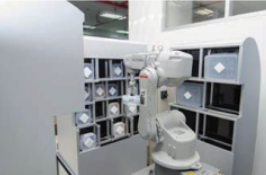
\includegraphics[width=3cm]{pics/thesis/table3.png}} \\
\hline

\cite{47} & 
An automated pill dispenser with a user-friendly interface to assist patients in managing medication intake through reminders, feedback, and interaction. & 
User interface setup, reminder system & 
\raisebox{-1\height}{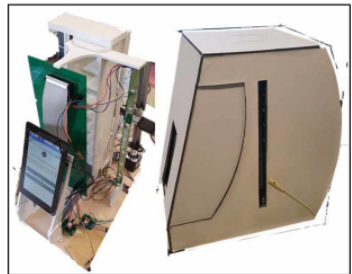
\includegraphics[width=3cm]{pics/thesis/table4.png}} \\
\hline

\end{tabular}
\end{table}


\section{ Comparative Evaluation of Medicine Adherence and Medical Bots in the Healthcare Sector}

Medication adherence is a key part of effective healthcare, especially for patients with chronic illnesses. Smart technologies like the Medication Event Monitoring System (MEMS\textsuperscript{\textregistered}) \cite{43}, RFID-enabled packaging, and IoT-integrated platforms such as I-CARES show promise in tackling adherence issues. They offer real-time monitoring, automated dispensing, and feedback mechanisms that involve both patients and caregivers \cite{48}. These systems track medication intake and provide alerts and health analytics. This support enables timely interventions and emergency responses. By improving patient engagement and allowing for proactive healthcare delivery, these innovations lower the chances of medication errors, cut healthcare costs, and enhance treatment outcomes. However, challenges with cost, scalability, and accessibility need to be addressed for wider use.
\begin{table}[h!]
\centering
\caption{Overview of Intelligent Medication Adherence and Medical bot Technologies along with Capabilities and Challenges}
\label{tab:adherence_tech}
\begin{tabular}{|p{1.5cm}|p{2.2cm}|p{3.5cm}|p{3.5cm}|p{3.3cm}|}
\hline
\textbf{Citation} & \textbf{System} & \textbf{Key Technologies} & \textbf{Strengths} & \textbf{Limitations} \\ \hline
\cite{49} & RxPense & IoT, real-time dashboards & Comprehensive monitoring, multi-user & Expensive, complex interface \\ \hline
\cite{50} & PillGood & Facial recognition, cloud monitoring & Highly secure, adaptive to user & Light sensitivity, power consumption \\ \hline
\cite{51} & MEDIC & Arduino-based, GSM alerts & Simple and effective, ideal for home use & No cloud-based tracking \\ \hline
\cite{52} & HearMe & NFC with text-to-speech synthesis & Accessible to visually impaired users & Requires precise tag alignment \\ \hline
\cite{53} & Advanced Dispenser & Automated dispensing pumps, digital control software, high-speed filling and sealing mechanisms, and barcoding and RFID tracking & Strong on security and remote access & Higher cost, requires technical setup \\ \hline
\end{tabular}
\end{table}

This comparison illustrates that most systems have strong capabilities; however, few can harness the strengths of cost, access, security, and multi-user features into one design. Thus it requires customizing based on the environment and user needs.

Research in robotics within elderly care has accelerated remarkably during the last decade. Three broad areas have been the focus: 1) Quality of life; 2) adherence and reports with healthcare access and medications, and 3) both emotional and physical aspects of interaction. The robotic systems rely on a wide range of technologies that permit voice recognition (speech), facial recognition, natural language processing (NLP), emotion detecting/detect, and autonomous movement; each of which ensures the robot interacts rather seamlessly while differentiating and assisting the user within their daily healthcare requirements. Many such robots are designed to work autonomously as required, therefore providing users with reliable and consistent support. The following table is a representation of important robotic systems that have been designed and constructed for elderly care settings. The table shows applications, algorithms or models underlying the systems, control, and the basic actions.

\begin{table}[htbp]
\centering
\caption{A compilation of the reference of smart Medora for elderly care.
}
\label{tab:library_interaction}
\begin{tabular}{|p{2cm}|p{10cm}|c|}
\hline
\textbf{Citation} & \textbf{Objective \& Application} & \textbf{Structure} \\ 
\hline
\cite{54}&
Development of Telepresence robots which can improve home healthcare for the elderly by reducing social isolation, enhancing safety, and providing remote access to healthcare services. These robots are used to support communication with family and caregivers, offer medication reminders, emergency alerts, and virtual consultations, and integrate with smart health devices for real-time monitoring to help elderly individuals live independently and safely at home.
 & \raisebox{-1\height}{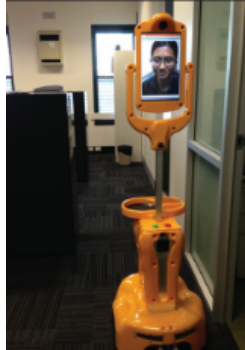
\includegraphics[width=3cm]{pics/thesis/table1.png}} \\ 
\hline
\cite{55} & 
This system aims to offer emotional support to the elderly through autonomous interaction using Natural Language Processing (NLP) and speech emotion recognition technologies. It engages users in meaningful conversations, detects their emotional states in real-time, and responds with appropriate verbal and non-verbal expressions to create a more empathetic and personalized experience. It system provides alerts and monitoring functions to ensure user safety and well-being, helping caregivers stay informed about the emotional and health status of elderly individuals.
 & \raisebox{-1\height}{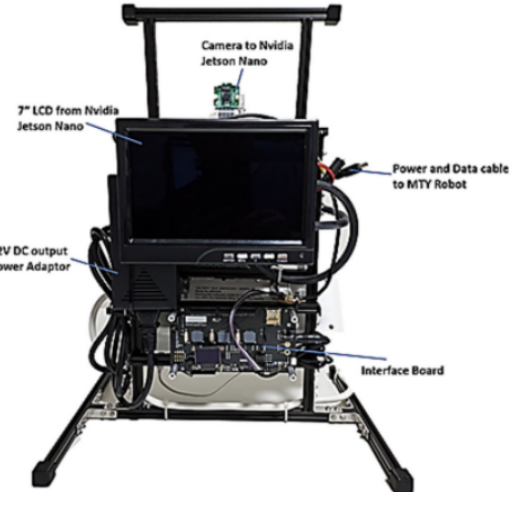
\includegraphics[width=3cm]{pics/thesis/SR.png}} \\ 
\hline
\cite{56} & Matilda is a social robot designed to support elderly care by providing emotional engagement, cognitive stimulation, and accessible interaction through voice, gesture, and facial recognition in nursing home settings.It helps reduce social isolation and supports residents with conditions like dementia and Parkinson’s disease. & \raisebox{-1\height}{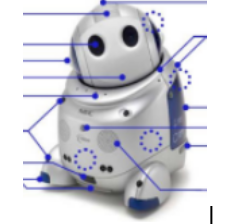
\includegraphics[width=3cm]{pics/thesis/tableM.png}} \\ 
\hline
\cite{57} & 
The robotic medication management system is designed to improve adherence in elderly home-care patients by automating medication schedules, reminders, dose verification, and lockout functions. It enables remote monitoring and alerts, ensuring timely and accurate dispensing while reducing the risk of missed or incorrect doses.
 & \raisebox{-1\height}{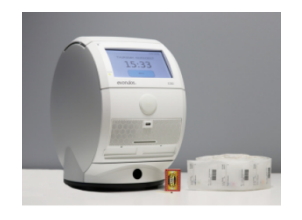
\includegraphics[width=4cm]{pics/thesis/table5.png}} \\ 
\hline
\end{tabular}
\end{table}
\FloatBarrier


Non-adherence to medication is an ongoing problem in healthcare for elderly and chronically ill patients and many have designed smart robotic dispensers to optimize the process of administering medications in an easier, faster, and usually more precise manner. Smart robotic dispensers implement technology such as, real-time medication monitoring, scheduling algorithms, inventory management, cloud synchronization, and user-centered concept designs. These techniques help to promote efficiency and efficacy, alongside every stage of the medication administration process. Most robotic/delivery systems operate autonomously, meaning they deliver reminders, confirmation of dose, and remote monitoring. The next table provides useful information about some of the selected robotic and smart dispensing systems, including the primary function, algorithms, form of control, and those it interacts with.

\section{Key Research Areas in Medication Management, Elderly Care, Emotion Detection, and Robotic Assistance}

Recent advances in healthcare technology emphasize integrated solutions for medication adherence, smart elder care, emotion detection, and communication systems—each of which contributes to the enhancement of patient health.

\textbf{Medication Adherence and Dispensing Systems} utilize innovations such as voice-controlled interfaces (e.g., Alexa skills), smart planners for the visually impaired, robotic medication dispensing systems, and integrated electronic prescriptions. These technologies aim to improve medication compliance and logistics in hospital settings. Despite these advantages, challenges remain in terms of cost-effectiveness and healthcare integration.

\textbf{Smart Homes and Elderly Care Support} incorporate IoT and machine learning to enable self-management in smart facilities, particularly benefiting rural and remote nursing homes. AI technologies, such as vision-based emotion detection and multimodal social robots, play a key role in enhancing the quality of elder care services.

\textbf{Emotion Detection and Social Robots} aim to identify emotional states through wearable sensors, voice analysis, and ambient intelligence. These technologies support patients—such as children with anxiety or individuals with dementia—by offering therapeutic interventions like empathetic robot interactions and music therapy.

\textbf{Voice Interaction and Communication Systems} include interactive voice response (IVR) and text-to-speech (TTS) platforms that deliver adaptive pharmaceutical guidance. These systems can enhance continuity of care by offering personalized directions and supporting healthcare compliance.

\begin{table}[h!]
\centering
\begin{tabular}{|p{4cm}|p{10.5cm}|}
\hline
\textbf{Citation(s)} & \textbf{Category and Function/Details} \\
\hline
\cite{58,59,60,61,62} & 
\textbf{Medication Adherence and Dispensing Systems:} Voice-controlled medication adherence via Alexa skill, smart planners for visually impaired, prototype robotic medication management, integrated e-prescribing with robotic dispensing, robotic drug storage and dispensing in hospital logistics. \\
\hline
\cite{63,64,65,66} & 
\textbf{Smart Homes and Elderly Care Support:} IoT and ML-based self-management systems for rural smart nursing homes, AI vision-based emotion detection for the elderly, multimodal social robots enhancing elderly care quality. \\
\hline
\cite{67,68,69} & 
\textbf{Emotion Detection and Social Robots:} Social robots providing safe emotional expression spaces for children with anxiety, ambient intelligent emotion detection using wearables, IoT-based speech emotion detection with deep learning, emotion monitoring and music interventions for dementia patients. \\
\hline
\cite{70} & 
\textbf{Voice Interaction and Communication Systems:} Interactive voice response and text-to-speech systems for adaptive pharmaceutical care. \\
\hline
\end{tabular}
\caption{Key Research Categories in Healthcare Technology}
\label{tab:key_areas}
\end{table}
